\section{Limits and Continuity}
A limit is when a function approaches, or gets infinitely close to a value. The standard notation for a limit is:
\[ \lim_{x \to c} f(x), \]
where $x$ approaches the value $c$ from both the left (negative values) or right (positive values).

\subsection{Sided Limits}
By adding a sign superscript to the $c$, it symbolizes that $x$ can only approach from the respective direction. A right-hand limit is when $x$ approaches $c$ from values greater than $c$:
\[ \lim_{x \to c^+} f(x). \]
Similarly, a left-hand limit is when $x$ approaches $c$ from values less than $c$:
\[ \lim_{x \to c^-} f(x). \]

It is important to note that a sided limit only exists if the function itself exists on that side of the value. More specifically,
$\lim \limits_{x \to c^+} f(x)$ only exists given $f(x) \in \R$ for all $x > c$, and $\lim \limits_{x \to c^-} f(x)$ only exists given $f(x) \in \R$ for all $x < c$. An example of this is:
\[ \lim_{x \to 0^-} \sqrt{x} = \text{undef} \]
because the function $\sqrt{x}$ does not exist for $x < 0$.

\subsection{Limits to Infinity}
If a degree of a polynomial is greater than or equal to $1$, its limit as $x$ approaches $\pm \infty$ will also be $\pm \infty$. The limit depends on the sign of the leading coefficient and the degree of the polynomial. For example:
\begin{align*}
	\lim_{x \to \infty} 2 x^3 - 7x^2 + 2 &= \infty   \\
	\lim_{x \to -\infty} 2 x^3 - 7x^2 + 2 &= -\infty.
\end{align*}
Here, the degree of the polynomial is $3$, and the leading coefficient, $2$, is positive. The function generally increases as $x$ increases.

When dealing with fractions of polynomials, if the degree of the numerator is greater than that of the denominator, the limit will be $\pm \infty$. In order to determine the sign of the limit, subtract the degree of the denominator from that of the numerator. For example,
\begin{align*}
	\lim_{x \to \infty} \frac{x^3 + 5}{x - 2} &= \infty   \\
	\lim_{x \to -\infty} \frac{3x^2 - 3}{x + 1} &= -\infty.
\end{align*}
When the degree of the denominator is higher than that of the numerator, the limit is always $0$. Methods for when the degrees are the same will be discussed later.

\subsection{Asymptotes}
\begin{figure}[H]
	\begin{center}
		\frame{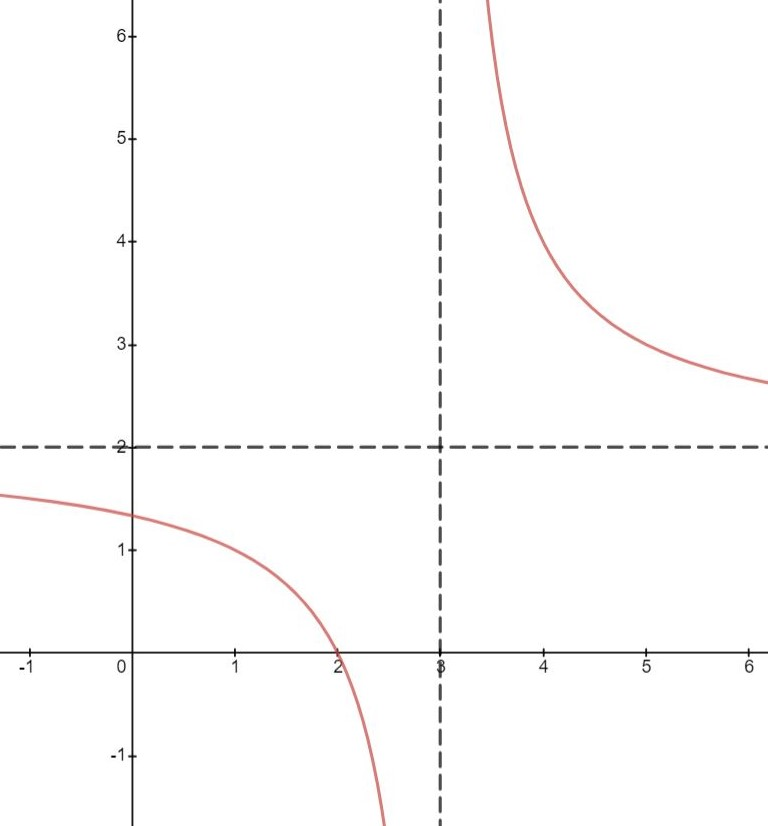
\includegraphics[width=0.5\textwidth]{fig1.JPG}}
		\caption{A function with horizontal and vertical asymptotes.}
		\label{fig:limasymptote}
	\end{center}
\end{figure}

When functions have vertical asymptotes, the limit as $x$ approaches it would be either $\infty$ or $-\infty$. It can also be undefined if the right and left sided limits have opposite signs. For example, given the function in Figure \ref{fig:limasymptote}:
\[ f(x) = \frac{2x-4}{x-3}, \]
its limits as $x \to 3$ are as follows:
\begin{align*}
	\lim_{x \to 3} & f(x) = \text{undef} \\
	\lim_{x \to 3^-} & f(x) = -\infty      \\
	\lim_{x \to 3^+} & f(x) = \infty
\end{align*}

As with horizontal asymptotes, as $x$ approaches $\pm \infty$, the function eventually gets very close to the value of the asymptote. Although the function, by definition, never touches the asymptote, the limit is equal to the $y$ value of the asymptote. Therefore:
\begin{align*}
	\lim_{x \to \infty} & f(x) = 2 \\
	\lim_{x \to -\infty} & f(x) = 2
\end{align*}

\subsection{Limit Properties}
\begin{figure}[H]
	\begin{center}
		\frame{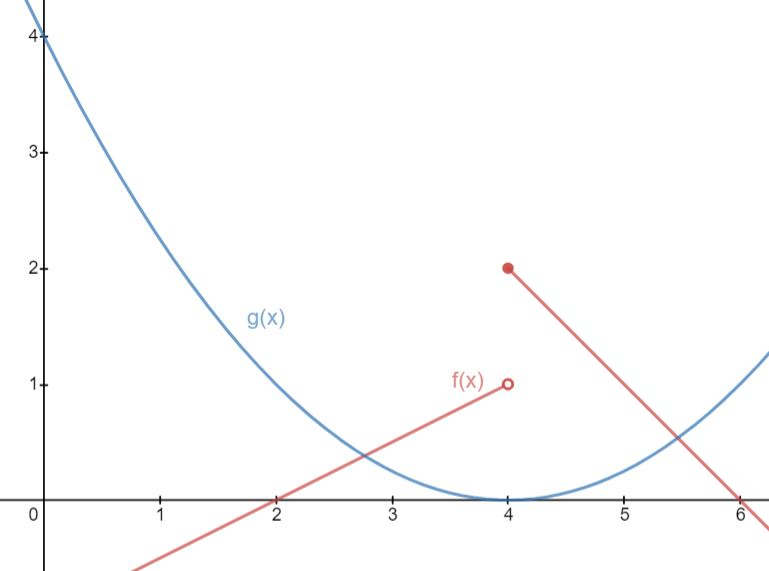
\includegraphics[scale=0.5]{fig2.JPG}}
		\caption{Two functions, $f(x)$ and $g(x)$.}
		\label{fig:limproperties}
	\end{center}
\end{figure}

Several rules can be applied when finding the limit of combined functions. The following examples are all based on Figure \ref{fig:limproperties}.

\subsubsection{Addition and Subtraction}
The combined limit of the sum or difference of two functions is equivalent to the sum or difference of the separate limits. In other words:
\[ \lim_{x \to c} \left[ f(x) \pm g(x) \right] = \lim_{x \to c} f(x) \pm \lim_{x \to c} g(x). \]
Applying this rule to the two functions in Figure \ref{fig:limproperties}:
\begin{align*}
	\lim_{x \to 2} \left[ f(x) + g(x) \right] &= \lim_{x \to 2} f(x) + \lim_{x \to 2} g(x) \\
	&= 0 + 1 \\
	\lim_{x \to 2} \left[ f(x) + g(x) \right] &= 1 \\[10pt]
	\lim_{x \to 2} \left[ g(x) - f(x) \right] &= \lim_{x \to 2} g(x) - \lim_{x \to 2} f(x) \\
	&= 1 - 0 \\
	\lim_{x \to 2} \left[ g(x) - f(x) \right] &= 1 \\[10pt]
	\lim_{x \to 4} \left[ f(x) + g(x) \right] &= \lim_{x \to 4} f(x) + \lim_{x \to 4} g(x) \\
	&= \text{undef} + 0 \\
	&= \text{undef}
\end{align*}

Note that in the last example, because the right and left side limits of $f(x)$ are not the same, its limit at $x = 4$ is \textit{undefined}. When adding $f(x)$ and $g(x)$, if just one of the functions has an undefined limit, the combined limit would also be undefined.

A generalization of the addition and subtraction properties for more than two functions is defined by the \textit{extended sum rule}. It states that:
\[ \lim_{x \to c} \left[ \sum_i f_i(x) \right] = \sum_i \left[ \lim_{x \to c} f_i(x) \right]. \]
Or in expanded notation:
\[ \lim_{x \to c} \left[ f_1(x) + \cdots + f_n(x) \right] = \lim_{x \to c} f_1(x) + \cdots + \lim_{x \to c} f_n(x). \]

\subsubsection{Multiplication}
Similar to addition and subtraction, the product of two functions is equivalent to the product of the separate limits. In other words:
\[ \lim_{x \to c} \left[ f(x) g(x) \right] = \lim_{x \to c} f(x) \lim_{x \to c} g(x). \]
Applying this rule to the two functions in Figure \ref{fig:limproperties}:
\begin{align*}
	\lim_{x \to 2} \left[ f(x) g(x) \right]
	&= \lim_{x \to 2} f(x) \cdot \lim_{x \to 2} g(x) \\
	&= 0 \cdot 2 \\
	&= 0
\end{align*}
The same exception applies when one of the limits is \textit{undefined}. This just makes the entire product's limit undefined.

A generalization of the product rule for more than two functions is defined by the \textit{extended product rule}, and is quite similar to the extended sum rule. It states that:
\[ \lim_{x \to c} \left[ \prod_i f_i(x) \right] = \prod_i \left[ \lim_{x \to c} f_i(x) \right]. \]
Or in expanded notation:
\[ \lim_{x \to c} \left[ f_1(x) f_2(x) \cdots f_n(x) \right] = \lim_{x \to c} f_1(x) \times \lim_{x \to c} f_2(x) \cdots \lim_{x \to c} f_n(x). \]

\subsubsection{Division}
In similar fashion, the quotient of two functions is equivalent to the quotient of the separate limits, as long as the limit of the denominator is not $0$. In other words:
\[ \lim_{x \to c} \frac{f(x)}{g(x)} = \frac{\lim_{x \to c} f(x)}{\lim_{x \to c} g(x)} \Rightarrow \lim_{x \to c} g(x) \ne 0. \]
Applying this rule to the two functions in Figure \ref{fig:limproperties}:
\begin{align*}
	\lim_{x \to 2} \frac{g(x)}{f(x)} &= \frac{\lim_{x \to 2} g(x)}{\lim_{x \to 2} f(x)} \\
	&= \frac{1}{0} \\
	&= \text{undef}
\end{align*}

\subsubsection{Composite Functions}
When finding the limit of a composite function, such as $f\left( g(x) \right)$, first evaluate the limit of the inner function, then evaluate the outer function normally. Hence:
\[ \lim_{x \to c} f\left( g(x) \right) = f\left( \lim_{x \to c} g(x) \right). \]
Applying this rule to the two functions in Figure \ref{fig:limproperties}:
\begin{align*}
	\lim_{x \to 1} f\left( g(x) \right) &= f\left( \lim_{x \to 1} g(x) \right) \\
	&= f(2) \\
	&= 0
\end{align*}
When the limit of the inner function is undefined, the limit of the composite equation would also be undefined. This is because the outer function does not exist at an undefined point.
\begin{align*}
	\lim_{x \to 4} g\left( f(x) \right) &= g\left( \lim_{x \to 4} f(x) \right) \\
	&= g(\text{undef}) \\
	&= \text{undef}
\end{align*}

\subsubsection{Constants}
Given that $\lim \limits_{x \to c} f(x)$ and $\lim \limits_{x \to c} g(x)$ are both finite for all $c \in \R$, then the following two equations hold:
\begin{gather*}
	\lim_{x \to c} k f(x) = k \lim_{x \to c} f(x) \\
	\lim_{x \to c} A = A
\end{gather*}
where $k$ and $A$ are both constants.

\subsection{Solving Limits}
There are several methods that can be used to solve a limit depending on various outcomes such as undefined solutions or indeterminate forms. These are outlined below.

\subsubsection{Direct Substitution}
The first method to try when solving a limit is \textbf{direct substitution}. For example:
\[ \lim_{x \to 6} -x^2 = -6^2 = -36. \]

There are two cases for when direct substitution will not work. The first of which is when it results in an undefined solution in the form $\frac{k}{0}$, where $k \in \R$. This means that there is likely an asymptote, and further methods can be used to determine a definite solution. The second of which is in the form $\frac{0}{0}$, which is called an \textit{indeterminate form}. This can be solved using either algebraic manipulation or L'Hopital's rule, to be mentioned later.

\subsubsection{Algebraic Manipulation}
When direct substitution results in an undefined value, the next method to try is algebraic manipulation. Such a method can involve factoring or polynomial division. For example:
\begin{align*}
	\lim_{x \to 2} \frac{x^4 + 3x^3 - 10x^2}{x^2 - 2x} & = \lim_{x \to 2} \frac{x^2 (x + 5)(x - 2)}{x(x - 2)} \\[5pt]
	&= \lim_{x \to 2} x(x + 5) \\
	&= 14
\end{align*}

However, not all functions can be factored. In these cases, if direct substitution does not work, the limit will evaluate to be undefined. For example:
\begin{align*}
	\lim_{x \to 1} \frac{2x}{x^2 - 7x + 6} &= \lim_{x \to 1} \frac{2x}{(x-6)(x-1)} \\
	&= \frac{2}{0} \\
	&= \text{undef}
\end{align*}

\subsubsection{Trigonometric Identities}
Trig identities can be used when dealing with trig equations, and direct substitution does not work. It will be useful to know the basic identities, among other ones:
\begin{table}[H]
	\centering
	\begin{tabular}{|c|c|}
		\hline
		\textbf{Pythagorean's identity} & $\sin^2(x) + \cos^2(x) = 1$ \\
		\hline
		\multirow{4}{*}{\textbf{Double angle identities}} & $\sin(2x) = 2 \sin(x) \cos(x)$ \\
		& $\cos(2x) = \cos^2(x) - \sin^2(x)$ \\
		& $\cos(2x) = 2\cos^2(x) - 1$ \\
		& $\cos(2x) = 1 - 2\sin^2(x)$ \\
		\hline
		\multirow{3}{*}{\textbf{Reciprocal identities}} & $\csc(x) = \frac{1}{\sin(x)}$ \\[5pt]
		& $\sec(x) = \frac{1}{\cos(x)}$ \\[5pt]
		& $\cot(x) = \frac{1}{\tan(x)} = \frac{\cos(x)}{\sin(x)}$ \\[5pt]
		\hline
	\end{tabular}
\end{table}

An example of when trig identities can be used to solve a limit is the limit as $x \to \frac{\pi}{2}$ for the function $f(x) = \frac{\cot^2(x)}{1 - \sin(x)}$. If direct substitution is used, it results in an indeterminate form $\frac{0}{0}$. Therefore, the limit can be solved as follows:
\begin{align*}
	\lim_{x \to \frac{\pi}{2}} \frac{\cot^2(x)}{1 - \sin(x)} &= \lim_{x \to \frac{\pi}{2}} \frac{1}{1 - \sin(x)} \left( \frac{\cos(x)}{\sin(x)} \right)^2 \\[5pt]
	&= \lim_{x \to \frac{\pi}{2}} \frac{\cos^2(x)}{\sin^2(x) (1 - \sin(x))} \\[5pt]
	&= \lim_{x \to \frac{\pi}{2}} \frac{1 - \sin^2(x)}{\sin^2(x) (1 - \sin(x))} \\[5pt]
	&= \lim_{x \to \frac{\pi}{2}} \frac{(1 + \sin(x))(1 - \sin(x))}{\sin^2(x) (1 - \sin(x))} \\[5pt]
	&= \lim_{x \to \frac{\pi}{2}} \frac{1 + \sin(x)}{\sin^2(x)} , \, 1 - \sin(x) \ne 0 \\[5pt]
	&= 2
\end{align*}

\subsection{Continuity}
A function is continuous $f(x)$ is continuous at a point $x = c$ if:
\[ \lim_{x \to c} f(x) = f(c). \] % the definition for continuity in the previous version was faulty

A function is continuous over the interval $[a, b]$ if it is continuous at each point within the interval. Some examples of functions and the intervals for which they are continuous:
\begin{itemize}
	\item $\sqrt{x + 4}$ is continuous for all $x \in [-4, \infty)$.
	\item $\sqrt[5]{x}$ is continuous for all $x \in \R$.
	\item $\ln x$ is continuous for all $x \in [0, \infty)$.
	\item $\frac{1}{x - 3}$ is continuous for all $x \ne 3$.
\end{itemize}

In general, functions won't be continuous if they have a division by $0$, square root of a negative number, or logarithm of $0$. For example, find the values of $x$ for which $f(x) = \frac{3x + 4}{x^2 - 3x + 2}$ is not continuous. In this function, $f(x)$ is undefined if the denominator is $0$, therefore it is not continuous for when:
\begin{align*}
	x^2 - 3x + 2 &= 0 \\
	(x - 2)(x - 1) &= 0 \\
	x &= 1, \, 2
\end{align*}
Altogether, the function $f(x)$ is continuous for $x \in \R, x \ne 1, \, 2$.

\subsubsection{Removable Discontinuity}
A function has a point of removable discontinuity if the value at that point is either undefined, or different from the limit of the function at that point. A function $f(x)$ has removable discontinuity at a point $x = c$ if:
\[ f(x) = \begin{cases}
		g(x) & \text{if} \; x \ne c \\
		k    & \text{if} \; x = c
	\end{cases} \quad \text{where} \, \lim_{x \to c} f(x) = g(c).\]

An example of a function with removable discontinuity is the function $f(x) = \frac{x - 2}{x - 2}$. This function is undefined at $x = 2$, but resembles the function $y = 1$ everywhere else. It can therefore be rewritten as:
\[ f(x) = \begin{cases}
    1 & \text{if} \; x \ne 2 \\
    \text{undef} & \text{if} \; x = 2
\end{cases}. \]
Notice that the limit of $f(x)$ as $x$ approaches $2$ is equal to $1$. Hence, the function has removable discontinuity at $x = 2$.

\subsubsection{Jump Discontinuity}
A function has a point of jump discontinuity if that part of the graph ``jumps'' from one $y$ value to another on the same $x$. The sided limits of the function at the point $x$ both exist, but are not equal. For example, function $f(x)$ from \ref{fig:limproperties} has jump discontinuity at $x = 4$. It can be denoted as follows:
\[ f(x) = \begin{cases}
    \frac{x}{2} - 1 & \text{if} \; x < 4 \\
    -x + 6 & \text{if} \; x \ge 4
\end{cases}. \]

\subsubsection{Infinite Discontinuity}
A function has a point of infinite discontinuity if the $y$ value at a point $x$ approaches $\pm \infty$. This usually happens at a vertical asymptote. The sided limits both exist, and both approach $\pm \infty$. For example, the function $f(x) = \frac{1}{x}$ has infinite discontinuity at $x = 0$. This can be verified by:
\[ \lim_{x \to 0^-} f(x) = -\infty \quad \text{and} \quad \lim_{x \to 0^+} f(x) = \infty. \]

\subsection{Squeeze Theorem}
The squeeze theorem, also known as the sandwich theorem, can be used to find the limit of a function at a particular value, especially when direct evaluation of the limit is difficult.

Given an open interval $I$ that includes a point $c$, where all points, and three functions within the interval such that:
\[ f(x) \le g(x) \le h(x), \]
for every $x$ in $I$ not equal to $c$, and that:
\[ \lim_{x \to c} f(x) = \lim_{x \to c} h(x) = L, \]
then $\lim \limits_{x \to c} g(x) = L$.

\noindent \textbf{Examples:}
\begin{enumerate}
    \item Find $\lim \limits_{x \to \infty} \frac{\sin x}{x}$.

    First, set up an inequality with the simpler part of the function, $\sin x$. The range of the $\sin x$ function is $[-1, 1]$. Therefore:
    \[ -1 \le \sin x \le 1. \]
    Next, divide the inequality by $x$ to resemble the original function:
    \[ -\frac{1}{x} \le \frac{\sin x}{x} \le \frac{1}{x}. \]
    Since $\lim \limits_{x \to \infty} -\frac{1}{x} = \lim \limits_{x \to \infty} \frac{1}{x} = 0$, by the squeeze theorem, $\lim \limits_{x \to \infty} \frac{\sin x}{x}$ must also be $0$. Therefore:
    \[ \lim \limits_{x \to \infty} \frac{\sin x}{x} = 0. \]

    \item Find $\lim \limits_{x \to -\infty} \frac{x^2 (\sin x + \cos^3 x)}{(x^2 + 1)(x - 3)}$.

	The part of this function that is most likely to have a range is $\sin x + \cos^3 x$. The ranges of $\sin x$ and $\cos x$ are both $[-1, 1]$. Therefore:
	\begin{gather*}
		-1 \le \sin x \le 1 \numberthis{\label{eq:sin_range}} \\
		-1 \le \cos x \le 1
	\end{gather*}
	Taking the cube of the second inequality:
	\[ -1 \le \cos^3 x \le 1 \numberthis{\label{eq:cos3_range}}. \]
	Adding inequalities \eqref{eq:sin_range} and \eqref{eq:cos3_range} gets the range of part of the numerator of the original function:
	\[ -2 \le \sin x + \cos^3 x \le 2. \]
	Next, multiply the inequality by $\frac{x^2}{(x^2 + 1)(x - 3)}$:
	\[ \frac{-2 x^2}{(x^2 + 1)(x - 3)} \le \sin x + \cos^3 x \le \frac{2 x^2}{(x^2 + 1)(x - 3)}. \]
	Since
	\[ \lim_{x \to -\infty}\frac{-2 x^2}{(x^2 + 1)(x - 3)} = 0 \quad \text{and} \quad \lim_{x \to -\infty}\frac{2 x^2}{(x^2 + 1)(x - 3)} = 0, \]
	by the squeeze theorem,
	\[ \lim_{x \to -\infty} \frac{x^2 (\sin x + \cos^3 x)}{(x^2 + 1)(x - 3)} = 0. \]
\end{enumerate}

\subsection{Intermediate Value Theorem}
Given a \textbf{continuous} segment of a function $f(x)$, let $c \in [a, b]$ and $w$ be in between $f(a)$ and $f(b)$. By the intermediate value theorem, there must be at least one value $c$ such that $f(c) = w$. That is, a continuous line in between points $A$ and $B$ must pass through every $x$ and $y$ value in between them. This goes both ways: if there is a $c$ then there is a $w$, and vice versa.

\begin{figure}[H]
	\begin{center}
		\frame{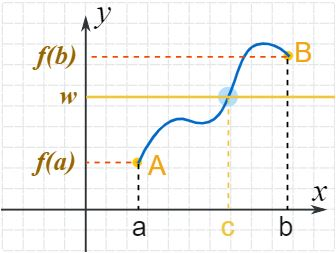
\includegraphics{images/fig3.JPG}}
	\end{center}
	\label{fig:inter_value_theorem}
	\caption{Visualization of the intermediate value theorem.}
\end{figure}